\documentclass[12pt]{article}

%%%%%%%%%%%%%%%%%%%%%%%%%%%%%%%%%%%%%%%%%%%%%%%%%%%%%%%%%%%%%%%%%%%%%%%%%%%%%%%%
%                           Package preset for homework
%%%%%%%%%%%%%%%%%%%%%%%%%%%%%%%%%%%%%%%%%%%%%%%%%%%%%%%%%%%%%%%%%%%%%%%%%%%%%%%%
% Miscellaneous
\usepackage[margin=1in]{geometry}
\usepackage[utf8]{inputenc}
\usepackage{indentfirst}
\usepackage{blindtext}
\usepackage{graphicx}
\usepackage{xr-hyper}
\usepackage{hyperref}
\usepackage{enumitem}
\usepackage{color}
\usepackage{float}
% Math
\usepackage{latexsym}
\usepackage{amsfonts}
\usepackage{amssymb}
\usepackage{amsmath}
\usepackage{commath}
\usepackage{amsthm}
\usepackage{bbold}
\usepackage{bm}
% Physics
\usepackage{physics}
\usepackage{siunitx}
% Code typesetting
\usepackage{listings}
% Citation
\usepackage[authoryear]{natbib}
\usepackage{appendix}
\usepackage[capitalize]{cleveref}
% Title & name
\title{Homework}
\author{Tien Vo}
\date{\today}


%%%%%%%%%%%%%%%%%%%%%%%%%%%%%%%%%%%%%%%%%%%%%%%%%%%%%%%%%%%%%%%%%%%%%%%%%%%%%%%%
%                   User-defined commands and environments
%%%%%%%%%%%%%%%%%%%%%%%%%%%%%%%%%%%%%%%%%%%%%%%%%%%%%%%%%%%%%%%%%%%%%%%%%%%%%%%%
%%% Misc
\sisetup{load-configurations=abbreviations}
\newcommand{\due}[1]{\date{Due: #1}}
\newcommand{\hint}{\textit{Hint}}
\let\oldt\t
\renewcommand{\t}[1]{\text{#1}}

%%% Bold sets & abbrv
\newcommand{\N}{\mathbb{N}}
\newcommand{\Z}{\mathbb{Z}}
\newcommand{\R}{\mathbb{R}}
\newcommand{\Q}{\mathbb{Q}}
\let\oldP\P
\renewcommand{\P}{\mathbb{P}}
\newcommand{\LL}{\mathcal{L}}
\newcommand{\FF}{\mathcal{F}}
\newcommand{\HH}{\mathcal{H}}
\newcommand{\NN}{\mathcal{N}}
\newcommand{\ZZ}{\mathcal{Z}}
\newcommand{\RN}[1]{\textup{\uppercase\expandafter{\romannumeral#1}}}
\newcommand{\ua}{\uparrow}
\newcommand{\da}{\downarrow}

%%% Unit vectors
\newcommand{\xhat}{\vb{\hat{x}}}
\newcommand{\yhat}{\vb{\hat{y}}}
\newcommand{\zhat}{\vb{\hat{z}}}
\newcommand{\nhat}{\vb{\hat{n}}}
\newcommand{\rhat}{\vb{\hat{r}}}
\newcommand{\phihat}{\bm{\hat{\phi}}}
\newcommand{\thetahat}{\bm{\hat{\theta}}}

%%% Other math stuff
\providecommand{\units}[1]{\,\ensuremath{\mathrm{#1}}\xspace}
% Set new style for problem
\newtheoremstyle{problemstyle}  % <name>
        {10pt}                   % <space above>
        {10pt}                   % <space below>
        {\normalfont}           % <body font>
        {}                      % <indent amount}
        {\bfseries\itshape}     % <theorem head font>
        {\normalfont\bfseries:} % <punctuation after theorem head>
        {.5em}                  % <space after theorem head>
        {}                      % <theorem head spec (can be left empty, 
                                % meaning `normal')>

% Set problem environment
\theoremstyle{problemstyle}
\newtheorem{problemenv}{Problem}[section]
\newenvironment{problem}[1]{%
  \renewcommand\theproblemenv{#1}%
  \problemenv
}{\endproblemenv}
% Set lemma environment
\newenvironment{lemma}[2][Lemma]{\begin{trivlist}
\item[\hskip \labelsep {\bfseries #1}\hskip \labelsep {\bfseries #2.}]}{\end{trivlist}}
% Set solution environment
\newenvironment{solution}{
    \begin{proof}[Solution]$ $\par\nobreak\ignorespaces
}{\end{proof}}
\numberwithin{equation}{problemenv}

%%% Page format
\setlength{\parindent}{0.5cm}
\setlength{\oddsidemargin}{0in}
\setlength{\textwidth}{6.5in}
\setlength{\textheight}{8.8in}
\setlength{\topmargin}{0in}
\setlength{\headheight}{18pt}

%%% Code environments
\definecolor{dkgreen}{rgb}{0,0.6,0}
\definecolor{gray}{rgb}{0.5,0.5,0.5}
\definecolor{mauve}{rgb}{0.58,0,0.82}
\lstset{frame=tb,
  language=Python,
  aboveskip=3mm,
  belowskip=3mm,
  showstringspaces=false,
  columns=flexible,
  basicstyle={\small\ttfamily},
  numbers=none,
  numberstyle=\tiny\color{gray},
  keywordstyle=\color{blue},
  commentstyle=\color{dkgreen},
  stringstyle=\color{mauve},
  breaklines=true,
  breakatwhitespace=true,
  tabsize=4
}
\lstset{
  language=Mathematica,
  numbers=left,
  numberstyle=\tiny\color{gray},
  numbersep=5pt,
  breaklines=true,
  captionpos={t},
  frame={lines},
  rulecolor=\color{black},
  framerule=0.5pt,
  columns=flexible,
  tabsize=2
}


\title{Homework 3: Astr 5140 (Fall 2021)}

\begin{document}
\maketitle
%%%%%%%%%%%%%%%%%%%%%%%%%%%%%%%%%%%%%%%%%%%%%%%%%%%%%%%%%%%%%%%%%%%%%%%%%%%%%%%%
\begin{problem}{1}[Generalized Ohm's Law]
The MHD force equation is derived by a linear combination of the electron and
ion fluid equations. Generalized Ohm's law is, simply stated, a different linear
combination.

We begin by multiplying the ion force equation by $m_e$ and the electron force
equation by $m_i$, then subtract
\begin{subequations}
    \begin{align}
        m_em_in\frac{D\vb{u}_i}{D t}
        &=-m_e\grad P_i+nm_ee(\vb{E}+\vb{u}_i\times\vb{B})
            -m_em_in\nu_{ie}(\vb{u}_i-\vb{u}_e)\\
        m_im_en\frac{D\vb{u}_e}{D t}
        &=-m_i\grad P_e-nm_ie(\vb{E}+\vb{u}_e\times\vb{B})
            -m_em_in\nu_{ei}(\vb{u}_e-\vb{u}_i)
    \end{align}
\end{subequations}
We use quasi-neutrality and bundle the convective derivative into the symbol
$D$.
\begin{align}
    m_em_in\qty(\frac{D\vb{u}_i}{Dt}-\frac{D\vb{u}_e}{Dt})
    &=\qty(-m_e\grad P_i+m_i\grad P_e)
    +en\vb{E}(m_e+m_i)\notag\\
    &\qquad+en\qty(m_e\vb{u}_i+m_i\vb{u}_e)\times\vb{B}
    -m_em_in(\nu_{ei}+\nu_{ie})(\vb{u}_i-\vb{u}_e)
\end{align}

(a) Divide each term by $en(m_i+m_e)$.

(b) Show that Term 1 can be re-written in the limit of $m_i\gg m_e$ as
\begin{equation}
    \frac{m_e}{e^2}\frac{D(\vb{J}/n)}{Dt} 
\end{equation}

(c) Argue that since $m_i\gg m_e$ that, unless $P_i\gg P_e$ (very rare), Term 2
becomes
\begin{equation}
    \frac{\grad P_e}{en} 
\end{equation}

(d) Term 3 is trivial. Term 4 is tricky as it must be broken into two parts. Add
$\vb{u}=(m_i\vb{u}_i+m_e\vb{u}_e) /(m_i+m_e)$, separate $\vb{u}\times\vb{B}$,
then subtract ($m_i\vb{u}_i+m_e\vb{u}_e) /(m_i+m_e)$. Show that the remaining
four terms ($m_i\gg m_e$) can be approximated as
\begin{equation}
    \frac{-\vb{J}\times\vb{B}}{en} 
\end{equation}

(e) Show that Term 5 can be written as $\vb{J}/\sigma$. Define $\sigma$.

In the end, you should arrive at
\begin{equation}
    \vb{E}+\vb{u}\times\vb{B}=\frac{\vb{J}}{\sigma}+\frac{\vb{J}\times\vb{B}}{en}-\frac{\grad
    P_e}{en}+\frac{m_e}{ne^2}\frac{D\vb{J}}{Dt}+\text{small terms} 
\end{equation}

\textbf{Note}: If done exactly (full convective derivative and keeping small
terms), $n$ is not inside the derivative and furthermore, some of the
''leftovers'' from Term 1 cancel ''leftovers'' in Term 4.
\begin{solution}
(a) Given the force equation with collisional terms,
\begin{equation}
    n_sm_s\frac{D\vb{u}_s}{Dt}=-\grad P_s+n_sq_s(\vb{E}+\vb{u}_s\times\vb{B})
    +m_sn_s\vb{g}
\end{equation}
we can write for ions and electrons (with collisional terms)
\begin{subequations}
    \begin{align}
        m_em_in\frac{D\vb{u}_i}{Dt}&=-m_e\grad
        P_i+m_ene(\vb{E}+\vb{u}_i\times\vb{B})+m_em_in\vb{g}
        -m_em_in\nu_{ie}(\vb{u}_i-\vb{u}_e)\label{p1a:ion}\\
        m_im_en\frac{D\vb{u}_e}{Dt}&=-m_i\grad
        P_e-m_ine(\vb{E}+\vb{u}_e\times\vb{B})+m_im_en\vb{g}
        -m_em_in\nu_{ei}(\vb{u}_e-\vb{u}_i)\label{p1a:electron}
    \end{align} 
\end{subequations}
where we have assumed a quasi-neutral plasma ($n_i=n_e=n$). Subtracting 
\eqref{p1a:ion} with \eqref{p1a:electron}, we get
\begin{align}
    m_im_en\frac{D}{Dt}(\vb{u}_i-\vb{u}_e)
    &=\qty(-m_e\grad P_i+m_i\grad P_e)+ne(m_i+m_e)\vb{E}\notag\\
    &\qquad+ne(m_e\vb{u}_i+m_i\vb{u}_e)\times\vb{B}
    -m_im_en(\nu_{ei}+\nu_{ie})(\vb{u}_i-\vb{u}_e)
\end{align}
Dividing each term by $en(m_i+m_e)$, we get
\begin{align}
    \frac1e\frac{m_im_e}{m_i+m_e}\frac{D}{Dt}(\vb{u}_i-\vb{u}_e)
    &=\frac1{en(m_i+m_e)}\qty(-m_e\grad P_i+m_i\grad P_e)+\vb{E}\notag\\
    &\qquad+\frac{m_e\vb{u}_i+m_i\vb{u}_e}{m_i+m_e}\times\vb{B}
    -\frac1e\frac{m_im_e}{m_i+m_e}(\nu_{ei}+\nu_{ie})(\vb{u}_i-\vb{u}_e)
\end{align}


(b) The current is $\vb{J}=en(\vb{u}_i-\vb{u}_e)$. Thus, we can rewrite the
first term as
\begin{equation}
    \frac1{e^2}\frac{m_im_e}{m_i+m_e}\frac{D(\vb{J}/n)}{Dt}
    =\frac{1}{e^2}\frac{m_e}{1+m_e/m_i}\frac{D(\vb{J}/n)}{Dt}
    \approx\frac{m_e}{e^2}\frac{D(\vb{J}/n)}{Dt}
\end{equation}
where $m_i\gg m_e$. Expanding the convective derivative, we can write
\begin{align}
    \frac{D(\vb{J}/n)}{Dt}
    &=\frac{\partial(\vb{J}/n)}{\partial
    t}+\vb{u}\vdot\grad\qty(\frac{\vb{J}}{n})\notag\\
    &=-\frac{\vb{J}}{n^2}\frac{\partial n}{\partial
    t}+\frac1n\frac{\partial\vb{J}}{\partial t}
+\vb{u}\vdot\qty[-\frac{\vb{J}}{n^2}\grad n+\frac1n\grad\vb{J}]\notag\\
    &=-\frac{\vb{J}}{n^2}\qty[\frac{\partial n}{\partial t}+\div{\qty(n\vb{u})}]
    +\frac1n\frac{\partial\vb{J}}{\partial t}
    +\frac1n\vb{u}\vdot\grad\vb{J}\notag\\
    &=\frac1n\frac{D\vb{J}}{Dt}
\end{align}

(c) The second term can be rewritten as
\begin{equation}
    \frac{1}{en}\qty[-\frac{m_e/m_i}{1+m_e/m_i}\grad
        P_i+\frac1{1+m_e/m_i}\grad P_e] 
    \approx\frac{\grad P_e}{en}
\end{equation}
where the first term vanishes when $m_e /m_i\ll 1$ unless $P_i\gg P_e$.

(d) Adding and subtracting $\vb{u}$ to the velocity, the fourth term is
\begin{align}
    \frac{m_e\vb{u}_i+m_i\vb{u}_e}{m_i+m_e}\times\vb{B}
    &=\qty[\vb{u}+\frac{m_e\vb{u}_i-m_i\vb{u}_e}{m_i+m_e}-\frac{m_i\vb{u}_i+m_e\vb{u}_e}{m_i+m_e}]\times\vb{B}\notag\\
    &=\qty[\vb{u}-\frac{m_i-m_e}{m_i+m_e}\qty(\vb{u}_i-\vb{u}_e)]\times\vb{B}
    \notag\\
    &\approx\vb{u}\times\vb{B}-\qty(\vb{u}_i-\vb{u}_e)\times\vb{B}\notag\\
    &=\vb{u}\times\vb{B}-\frac{\vb{J}\times\vb{B}}{en}
\end{align}

(e) Writing the last term in terms of the current, we get
\begin{align}
    -\frac1e\frac{m_im_e}{m_i+m_e}\qty(\nu_{ei}+\nu_{ie})\qty(\vb{u}_i-\vb{u}_e)
    =-\frac1{e^2n}\frac{m_e}{1+m_e/m_i}\qty(\nu_{ei}+\nu_{ie})\vb{J}
    =-\frac{m_e(\nu_{ei}+\nu_{ie})}{e^2n}\vb{J}
\end{align}
Defining $\sigma=e^2n /m_e(\nu_{ei}+\nu_{ie})$, it becomes $-\vb{J} /\sigma$.

Combining everything, we get
\begin{equation}
    \frac{m_e}{ne^2}\frac{D\vb{J}}{Dt}
    =\frac{\grad
    P_e}{en}+\vb{E}+\vb{u}\times\vb{B}-\frac{\vb{J}\times\vb{B}}{en}-\frac{\vb{J}}{\sigma}
\end{equation}
Rewriting this result yields the generalized Ohm's law
\begin{equation}
    \vb{E}+\vb{u}\times\vb{B}=\frac{\vb{J}}{\sigma}+\frac{\vb{J}\times\vb{B}}{en}-\frac{\grad
    P_e}{en}+\frac{m_e}{ne^2}\frac{D\vb{J}}{Dt} 
\end{equation}
\end{solution}
\end{problem}
%%%%%%%%%%%%%%%%%%%%%%%%%%%%%%%%%%%%%%%%%%%%%%%%%%%%%%%%%%%%%%%%%%%%%%%%%%%%%%%%    

%%%%%%%%%%%%%%%%%%%%%%%%%%%%%%%%%%%%%%%%%%%%%%%%%%%%%%%%%%%%%%%%%%%%%%%%%%%%%%%%
\begin{problem}{2}[Scale height in the solar corona]
The surface gravity of the Sun is $274$\,\si{m/s\tothe{2}}. Assume that the
corona is entirely protons with $T_{\text{corona}}=10^6$\,$^\circ$\si{K}.
Derive the isothermal scale height of the solar corona from the MHD equations
assuming $\vb{g}$ is constant (use 1D). How does this value compare with the
radius of the Sun (what \% of $R_{\text{sun}}$ is $H_0$)? Does your answer agree
with what is seen in UV or X-ray images?
\begin{solution}
The 1D state equation is
\begin{equation}
    \frac{\partial P}{\partial z}
    =\frac{\gamma T}{m}\frac{\partial\rho}{\partial z} 
\end{equation}
where $\gamma=1$ in an isothermal plasma and $T=k_BT_{\text{corona}}$. From the 
force equation, we can also write
\begin{equation}
    \frac{\partial P}{\partial z}=\rho g 
\end{equation}
Thus, we arrive at the following differential equation
\begin{equation}
    \frac{\partial n}{\partial z}=\frac{mg}{T}n 
\end{equation}
where $\rho=mn$. The solution is
\begin{equation}\label{p2:n}
    n=n_0e^{-mgz/T}=n_0e^{-z/H_0}
\end{equation}
where the scale height is $H_0=T /mg\approx 3\times 10^{4}$\,\si{km}. This is
$\approx 4\%$ of the Sun's radius. From EUVI images, the corona is usually 10s
of the scale height wide. But the density profile follows roughly the
exponential decay in \eqref{p2:n}.
\end{solution}
\end{problem}
%%%%%%%%%%%%%%%%%%%%%%%%%%%%%%%%%%%%%%%%%%%%%%%%%%%%%%%%%%%%%%%%%%%%%%%%%%%%%%%%
%%%%%%%%%%%%%%%%%%%%%%%%%%%%%%%%%%%%%%%%%%%%%%%%%%%%%%%%%%%%%%%%%%%%%%%%%%%%%%%%
\begin{problem}{3}[Force free flux rope]
Below are spacecraft observations of a force free flux rope passing by Earth
after a coronal mass ejection. The data are (a) the total magnetic field, (b)
the elevation angle from the solar ecliptic, (c) the azimuthal angle in the
solar ecliptic ($0^\circ$ indicates anti-sunward), (d) the plasma density, (e)
the thermal velocity, and (f) the solar wind speed.
\begin{center}
    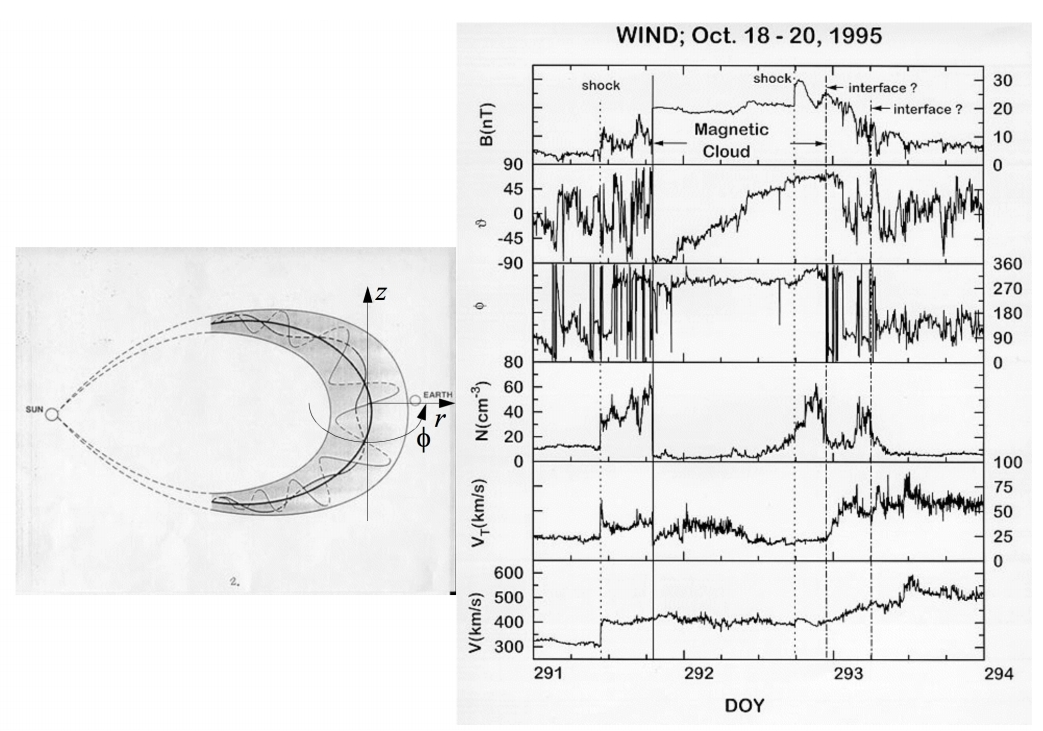
\includegraphics[width=0.8\textwidth]{hw3_p3.jpg} 
\end{center}
Unlike the force free flux rope in an earlier problem in which $\alpha$ was
constant, the observations indicate a steady rotation of the magnetic field (pay
particular attention to the second panel -- the elevation angle has a constant
slope) that is best modeled by assuming cylindrical symmetry with the $z$ axis
aligned with the flux rope (see the left diagram) and the magnetic field obeys
the relation: $B_\phi /B_z=\epsilon r$, where $\epsilon$ is a constant. Let the
magnetic field at the center be $B_z=B_0$.

(a) Under the force free equations with $\alpha$ NOT constant, show that
$\curl{\vb{B}}=\alpha\vb{B}$ can be expressed as
\begin{equation}
    \frac{\partial B_z}{\partial r}=-\alpha B_\phi
    \qquad\text{and}\qquad
    \frac1r\frac{\partial(rB_\phi)}{\partial r}=\alpha B_z
\end{equation}
Using the relationship $B_\phi /B_z=\epsilon r$, eliminate $B_\phi$ from the
above equations.

(b) Eliminate $\alpha$ by combining the two equations to obtain one differential
equation for $B_z$.

(c) Solve for $B_z$ with manipulation followed by direct integration. Also
derive $B_\phi$ and $\alpha$.

(d) Plot $B_z$ and $B_\phi$ a a function of $r$.
\begin{solution}
(a) Assume cylindrical symmetry, so $\partial\vb{B}/\partial\phi=0$. The curl of
$\vb{B}$ in cylindrical coordinates is
\begin{equation}
    \curl{\vb{B}}=-\frac{\partial B_\phi}{\partial z}\rhat
    -\frac{\partial B_z}{\partial r}\phihat
    +\frac1r\frac{\partial(rB_\phi)}{\partial r}\zhat
\end{equation}
Now, the force free equation is
$\curl{\vb{B}}=\alpha\vb{B}=\alpha(B_r\rhat+B_\phi\phihat+B_z\zhat)$. So we can 
write
\begin{equation}
    \frac{\partial B_z}{\partial r}=-\alpha B_\phi
    \qquad\text{and}\qquad
    \frac1r\frac{\partial(r B_\phi)}{\partial r}=\alpha B_z
\end{equation}
as desired. Since $B_\phi /B_z=\epsilon r$, we can eliminate $B_\phi$ from these
differential equations
\begin{equation}\label{p3a}
    \frac{\partial B_z}{\partial r}=-\alpha\epsilon rB_z
    \qquad\text{and}\qquad
    \frac{\epsilon}{r}\frac{\partial(r^2B_z)}{\partial r}=\alpha B_z
\end{equation}

(b) Combining the equations in \eqref{p3a}, we have
\begin{equation}\label{p3b}
    \frac{\partial B_z}{\partial r}=-\epsilon^2\frac{\partial
    (r^2B_z)}{\partial r}=-\epsilon^2\qty(2rB_z+r^2\frac{\partial
B_z}{\partial r})\Rightarrow
\qty(1+\epsilon^2r^2)\frac{\partial B_z}{\partial r}=-2\epsilon^2rB_z
\end{equation}

(c) The differential equation in \eqref{p3b} is separable into
\begin{equation}
    \frac{dB_z}{B_z}=-\frac{2\epsilon^2rdr}{1+\epsilon^2r^2} 
\end{equation}
Integrating both sides, we get
\begin{align}
    \ln B_z
    &=-\int\frac{2\epsilon^2rdr}{1+\epsilon^2r^2}\notag\\
    &=-\frac{du}{u}\tag{$u\equiv 1+\epsilon^2r^2$}\\
    &=-\ln\qty[B_0(1+\epsilon^2r^2)] 
\end{align}
So the solution is
\begin{equation}
    B_z=\frac{B_0}{1+\epsilon^2r^2} 
\end{equation}
Also, by the relation $B_\phi /B_z=\epsilon r$, we can write
\begin{equation}
    B_\phi=\frac{\epsilon r}{1+\epsilon^2r^2}B_0 
\end{equation}
Plugging this back into \eqref{p3a},
\begin{equation}
    \frac{\partial B_z}{\partial
    r}=-\frac{2\epsilon^2r}{(1+\epsilon^2r^2)^2}B_0
    =-\frac{\alpha\epsilon r}{1+\epsilon^2r^2}B_0
    \Rightarrow
    \alpha=\frac{2\epsilon}{1+\epsilon^2r^2}
\end{equation}

(d)
\begin{center}
    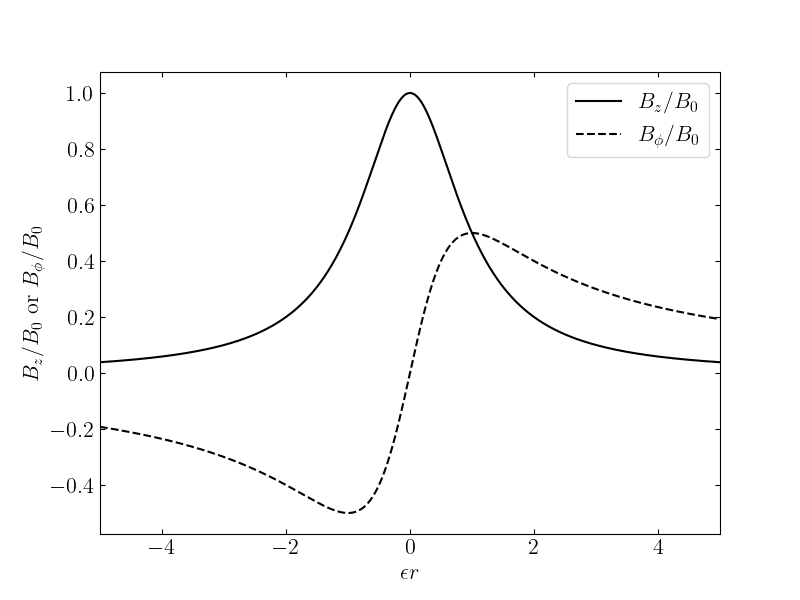
\includegraphics[width=1\textwidth]{p3.png} 
\end{center}
\end{solution}
\end{problem}
%%%%%%%%%%%%%%%%%%%%%%%%%%%%%%%%%%%%%%%%%%%%%%%%%%%%%%%%%%%%%%%%%%%%%%%%%%%%%%%%
%%%%%%%%%%%%%%%%%%%%%%%%%%%%%%%%%%%%%%%%%%%%%%%%%%%%%%%%%%%%%%%%%%%%%%%%%%%%%%%%
\begin{problem}{4}[Magnetic tension]
This problem is to develop an intuition for magnetic tension. Examine the
diagram, which shows a field line if $\vb{B}=B_0[(z /z_0)\xhat+\zhat]$. Examine
the field line and convince yourself that the equation represents a curved
magnetic field line. Derive the tension force at $z=0$. What is the direction of
the tension force? Argue that $z_0$ is the local radius of curvature.
\begin{center}
    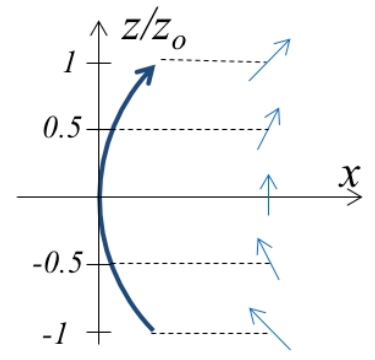
\includegraphics[width=0.3\textwidth]{hw3_p4.jpg} 
\end{center}
\begin{solution}
Given the magnetic field
\begin{equation}\label{p4}
    \vb{B}=B_0\qty(\frac{z}{z_0}\xhat+\zhat) 
\end{equation}
the tension force is, by definition
\begin{align}
    \frac1{\mu_0}\vb{B}\vdot\grad\vb{B}
    =\frac1{\mu_0}\qty[B_x\frac{\partial}{\partial
    x}+B_z\frac{\partial}{\partial z}]\vb{B}
    =\frac1{\mu_0}B_0\frac{B_0}{z_0}\xhat
    =\frac{B_0^2}{\mu_0}\frac1{z_0}\xhat
\end{align}
This tension force is constant and is in the $x$ direction.
\begin{center}
    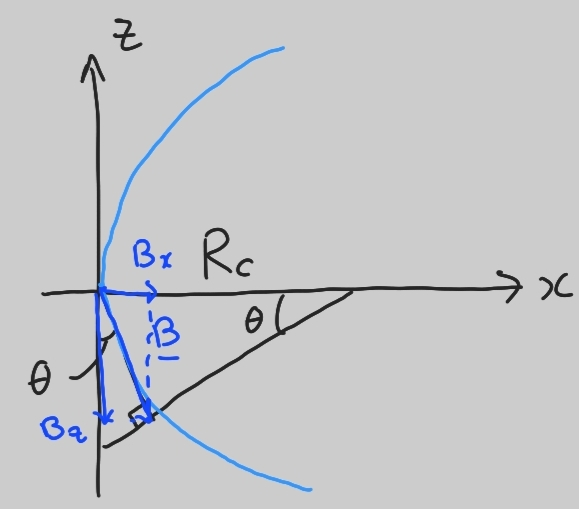
\includegraphics[width=0.3\textwidth]{hw3_p4b.jpg} 
\end{center}
Draw a point equidistant (for $z /z_0\ll 1$) to the magnetic field (blue) on the
$x$ axis at $R_c$ as above. If $\sin\theta\ll 1$, we can write by geometry that
\begin{equation}
    \tan\theta\approx\frac{B_x}{B_z}\approx\frac{z}{R_c} 
\end{equation}
But $B_x /B_z=z /z_0$ from \eqref{p4}. So $z /R_c=z /z_0\Rightarrow z_0=R_c$.
$z_0$ is thus the local radius of the curvature.
\end{solution}
\end{problem}
%%%%%%%%%%%%%%%%%%%%%%%%%%%%%%%%%%%%%%%%%%%%%%%%%%%%%%%%%%%%%%%%%%%%%%%%%%%%%%%%
%%%%%%%%%%%%%%%%%%%%%%%%%%%%%%%%%%%%%%%%%%%%%%%%%%%%%%%%%%%%%%%%%%%%%%%%%%%%%%%%
\begin{problem}{5}[Pulsars]
Radio signals that we receive from space not only give us information about the
source but can tell us about the interstellar medium. For example, impulsive
signals can show strong frequency dispersion as diagramed below.
\begin{center}
    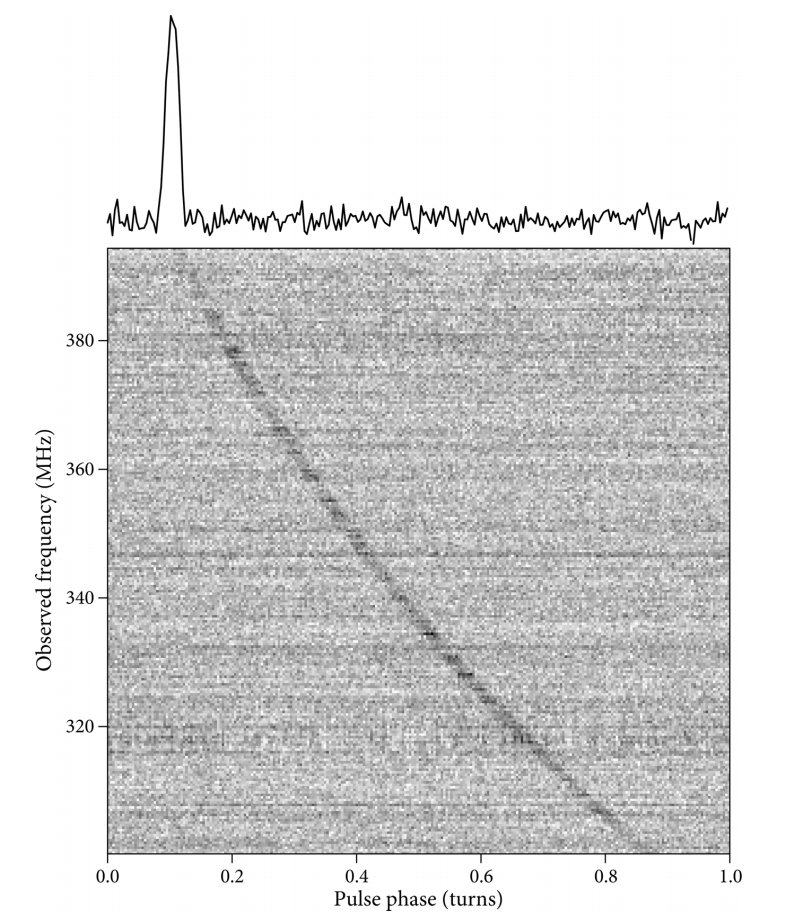
\includegraphics[width=0.6\textwidth]{hw3_p5.jpg}
\end{center}

(a) We showed that the solution of a transverse light wave becomes
$\omega^2=c^2k^2+\omega_{pe}^2$. Derive the group velocity $d\omega /dk$ of the
light wave.

(b) Assuming that $\omega\gg\omega_{pe}$, show that the ``delay'' (from
light-speed) it takes to travel a distance $L$ is, to lowest order, is directly
proportional to $n_eL$, the total electron content (column electron density).
Derive an expression for the time delay in terms of $\omega$ and $n_eL$.

(c) Describe (in words is OK) how one can determine the average density of the
interstellar medium from a pulsar frequency dispersion.
\begin{solution}
(a) Taking the implicit differentiation of the dispersion relation, we get
\begin{equation}
    2\omega d\omega=2c^2kdk\Rightarrow v_g=\frac{d\omega}{dk}
    =\frac{c}{\omega/k}=c\qty(1+\frac{\omega_{pe}^2}{c^2k^2})^{-1/2}
\end{equation}
where $v_g$ is the group velocity of the light wave.

(b) If $\omega\gg\omega_{pe}$, then from the dispersion relation,
\begin{equation}
    1=\frac{c^2k^2}{\omega^2}+\frac{\omega_{pe}^2}{\omega^2}
    \approx\frac{c^2k^2}{\omega^2}
\end{equation}
We can then approximate the group velocity as
\begin{equation}
    v_g\approx c\qty(1-\frac12\frac{\omega_{pe}^2}{\omega^2}) 
\end{equation}
The travel time is then
\begin{equation}
    \tau=\frac{L}{v_g}\approx\frac{L}{c}\qty(1+\frac12\frac{\omega_{pe}^2}{\omega^2})
\end{equation}
So the delay is 
\begin{equation}\label{p5b:delay}
    \tau_{\text{delay}}=\tau-\tau_{\omega\to\infty}
    =\frac{L}{2c}\frac{\omega_{pe}^2}{\omega^2}
    =\frac{e^2}{2c\epsilon_0m_e}\frac{\expval{n_e}L}{\omega^2}
\end{equation}
where $\expval{n_e}L=\int_0^Ln(s)ds$ is the total electron content.

(c) From \eqref{p5b:delay}, we can write
\begin{equation}
    \expval{n_e}=\frac{2\epsilon_0m_e\omega^2}{e^2}\frac{c\tau_{\text{delay}}}{L} 
\end{equation}
The average electron density can thus be determined from the delay time, the
interstellar distance $L$, and the frequency $\omega$ through the above
expression. One can approximate where $\tau_{\omega\to\infty}$ is in the graph
and pick a point of finite frequency on the drifted power curve in the 
spectrogram to calculate the delay time.
\end{solution}
\end{problem}
%%%%%%%%%%%%%%%%%%%%%%%%%%%%%%%%%%%%%%%%%%%%%%%%%%%%%%%%%%%%%%%%%%%%%%%%%%%%%%%%

\end{document}
